\subsection{Aggiunta Pannello alla Dashboard}\label{AddPanel}

Una volta effetuato l'accesso a \textit{Grafana} è necessario per prima cosa aggiungere alla propria Dashboard il pannello \textit{G\&B}. Gli utenti con esperienza nell'uso della piattaforma \textit{Grafana} non dovrebbero aver problemi in tal senso, ciò nonostante forniamo una descrione di questa operazione per chi ne avesse bisogno.\\

\begin{figure}[H]
	\begin{center}
		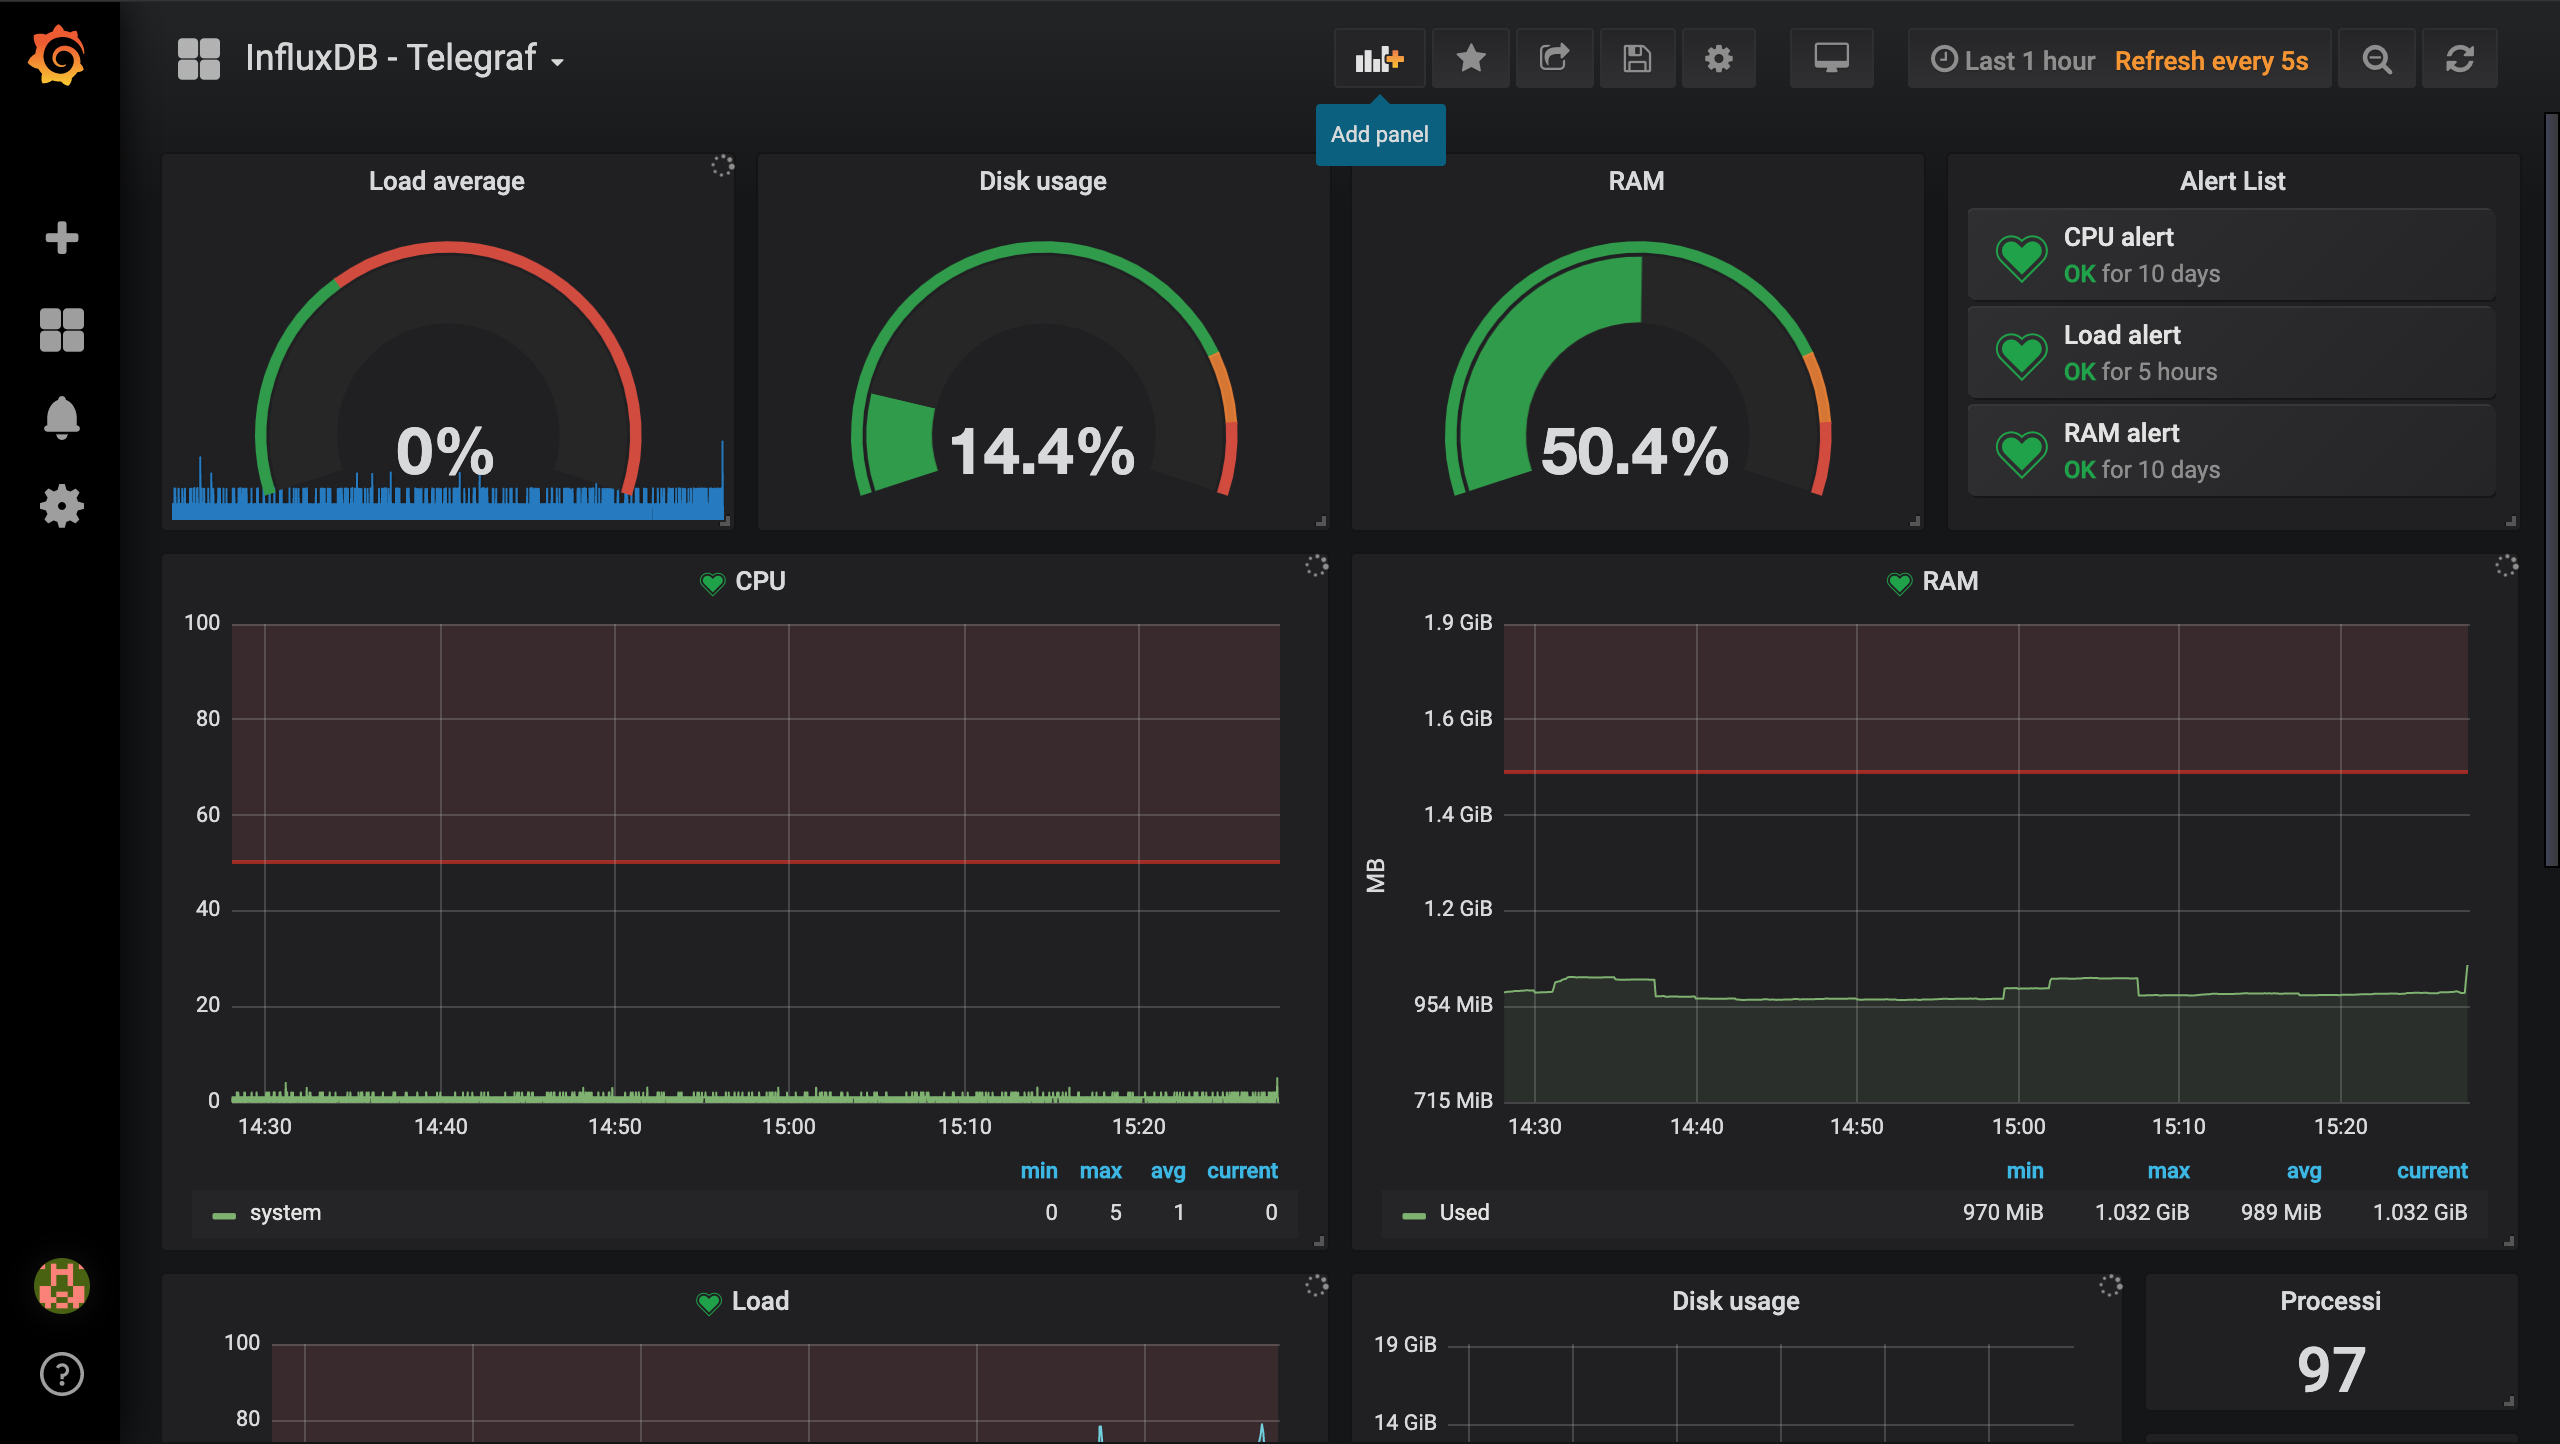
\includegraphics[scale=0.33]{./images/Dashboard.png}
		 \caption{Dashboard di esempio della piattaforma Grafana}	
		 \label{Dashboard}
	\end{center}
\end{figure}

La Figura \ref{Dashboard} espone una Dashboard di esempio, con evidenziato il dettaglio dell'hover causato dal mouse posizionato sul pulsante \textbf{Add panel}.\\
L'operazione di aggiunta del pannello si compone di due semplice passaggi:
~\\

\textbf{PASSAGGIO 1:} L'utente clicca il pulsante "Add panel" posizionato centralmente nella parte superiore della dashboard. Nella Figura \ref{Dashboard} è visibile l'effetto di hover di tale pulsante.
~\\

\textbf{PASSAGGIO 2:} L'utente,  che ora visualizza la finestra di aggiunta di un pannello, deve spostarsi nella sezione \textbf{Add} e selezionare il pannello \textit{G\&B} (Figura \ref{AddPanelImg}).

\begin{figure}[H]
	\begin{center}
		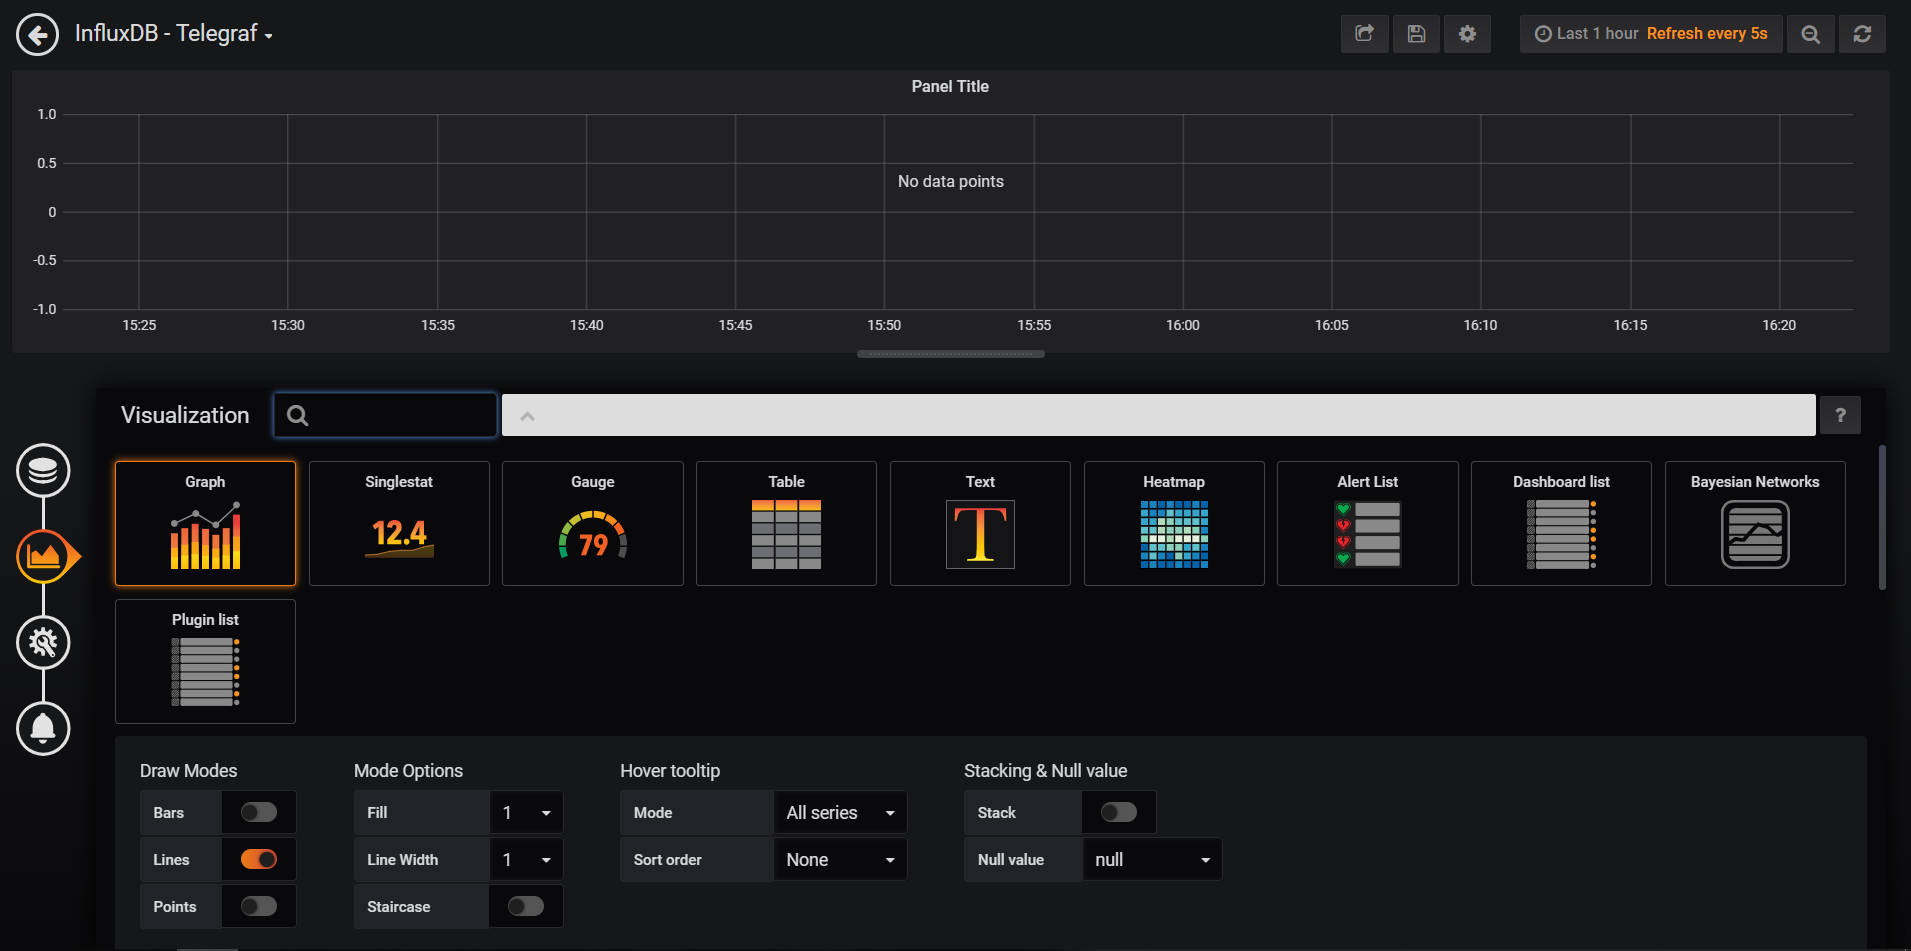
\includegraphics[scale=0.33]{./images/AddPanel.png}
		 \caption{Finestra di selezione del pannello da aggiungere alla propria Dashboard}	
		 \label{AddPanelImg}
	\end{center}
\end{figure}


Una volta selezionato il pannello sarà aggiunto alla Dashboard dell'utente, come si può vedere in Figura \ref{DashboardPanel}.

\begin{figure}[H]
	\begin{center}
		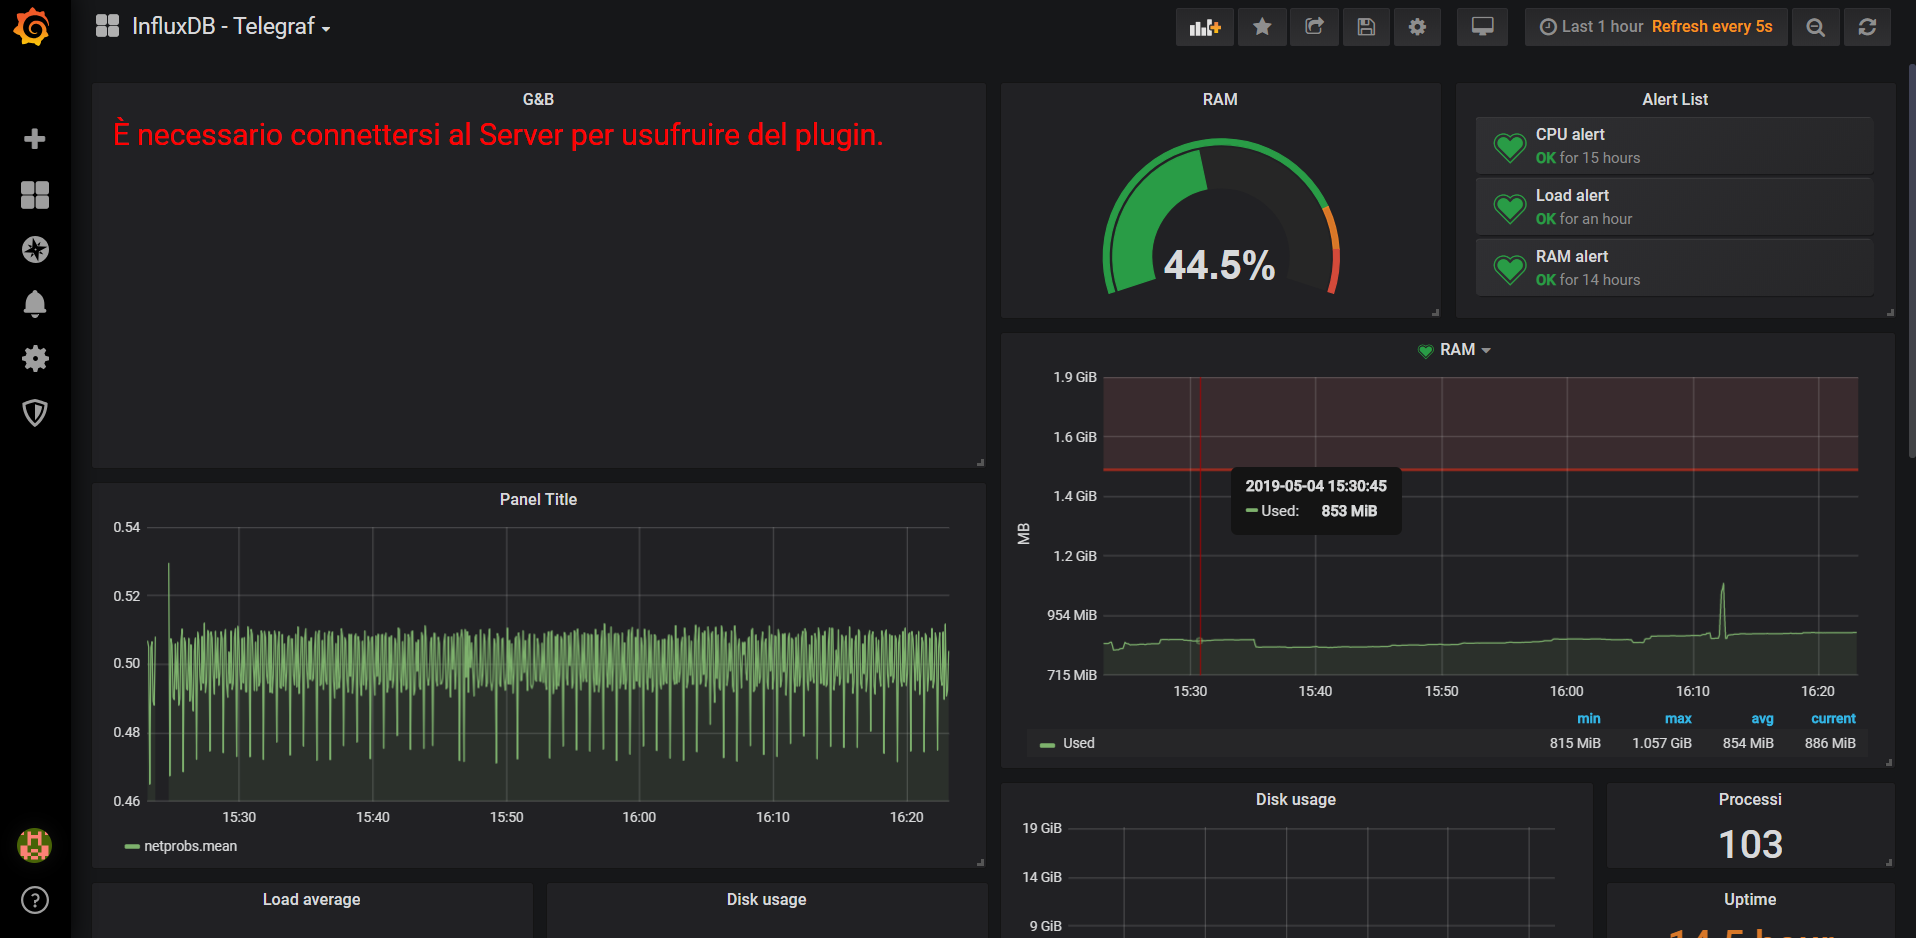
\includegraphics[scale=0.33]{./images/DashboardPanel.png}
		 \caption{Dashboard di Grafana contente il pannello G\&B}	
		 \label{DashboardPanel}
	\end{center}
\end{figure}
